\section{Auswertung und Diskussion}
\label{sec:AuswertungDiskussion}

\subsection*{Bestrahlungsplan für das PTV1}
Bei der ersten Serie wird das PTV1 bestrahlt. In den Abbildungen \ref{fig:lunge1x}, \ref{fig:lunge1y} und \ref{fig:lunge1z} ist die Dosisverteilung in der Lunge in der
Transversal-, Sagittal- und Frontalansicht zu sehen. In den Abbildungen ist zu erkennen, dass die $\SI{95}{\percent}$ Isodosenlinie das
rot eingezeichnete PTV in dem meisten Bereichen recht gut umschließt, obwohl das PTV1 relativ groß ist.
Für eine bessere Beurteilung ist das Dosis-Volumen-Histogramm in der Abbildung \ref{fig:lunge1dvh} gezeigt.
Es ist lediglich in einem kleinen Teil des PTVs nicht gelungen eine Dosis von $\SI{95}{\percent}$ zu erreichen. Das liegt daran, dass das PTV sehr nah am Herz liegt und sie wird durch die MLCs geschützt. Aus diesem Grund lässt sich keine relative Dosis von $\SI{95}{\percent}$ erreichen. Es werden also $\SI{95,25}{\percent}$ von der $\SI{95}{\percent}$ Isodosenlinie umschlossen.
Außerdem ergibt sich eine maximale Dosis von $\SI{105.3}{\percent}$, welche um ungefähr $\SI{2}{\percent}$ unter der erlaubten maximalen Dosis von $\SI{107}{\percent}$ liegt und sich innerhalb des PTVs befindet. Die minimale Dosis, die im PTV deponiert wird, liegt bei $\SI{86.2}{\percent}$.
Es konnte auch schon anhand der Dosisverteilungen gesehen werden, dass nicht im gesamten PTV eine relative Dosis von $\SI{95}{\percent}$ erreicht werden konnte. Die Lungen, das Herz sowie das Rückenmark müssen so gut wie möglich geschont werden.
Es wäre möglich durch die Änderung der Gantry-Rotationen oder der MLCs, dass das PTV besser umschlossen wird. Dadurch können aber die Risikoorgane mehr Dosis bekommen und hierbei müssen die Organdosisgrenzwerte in der ersten als auch in der zweiten Serie berücksichtigt werden.

\begin{figure}[H]
	\centering
	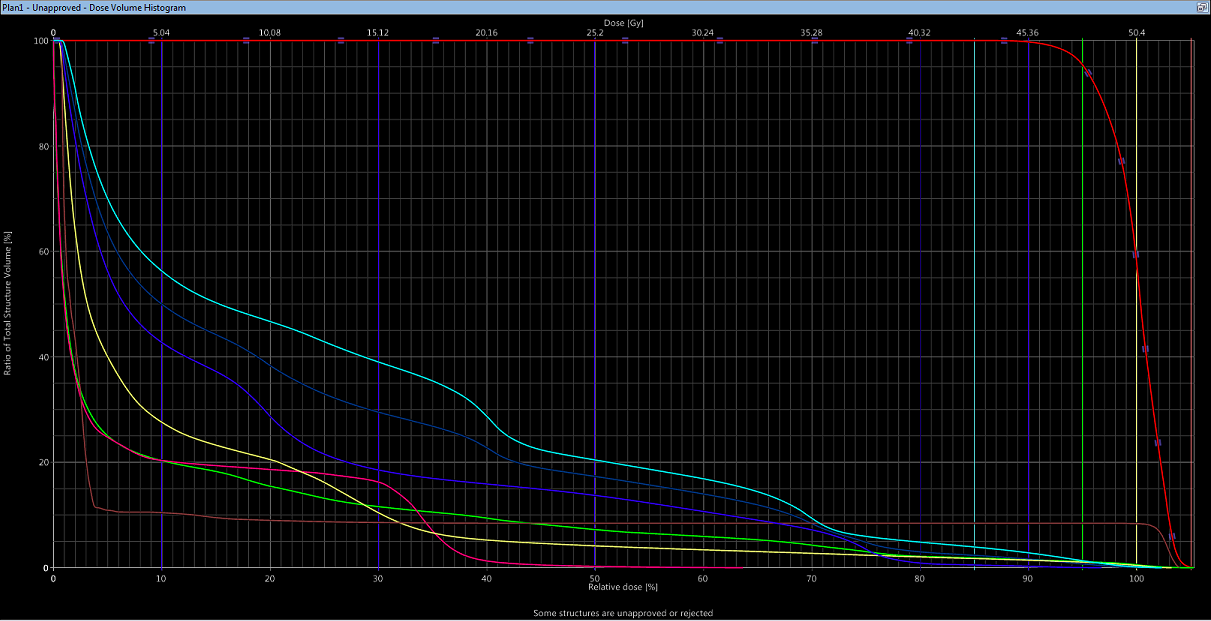
\includegraphics[width=\linewidth]{Bilder/Lunge1_DVH}
	\caption{Zu sehen ist das DVH der Lunge. In roter Farbe dargestellt ist das PTV1 und in grüner Farbe ist der Body. Außerdem sind noch die einzelnen Isodosenlinien eingezeichnet und die einzelnen Kurven zu den Risikoorgane wie z.B. Herz(gelb), Lunge(dunkelblau), die Speiseröhre(braun) und das Rückenmark(pink).}
	\label{fig:lunge1dvh}
\end{figure}

Anhand des DVHs des gesamten Körpers (grüne Kurve) ist zu erkennen, dass der Körper nur eine relativ geringe Dosis deponiert wird. Nur etwa $\SI{7,22}{\percent}$ des Körpervolumens erhält noch eine relative Dosis von $\SI{50}{\percent}$, dass obwohl das PTV1 recht groß ist. Um zu überprüfen ob die Organdosisgrenzwerte eingehalten worden sind, müssen beide Bestrahlungspläne betrachtet werden. Aus diesem Grund wird die Dosisverteilung der Risikoorgane am Ende des Protokolls genauer untersucht.

\begin{figure}[H]
	\centering
	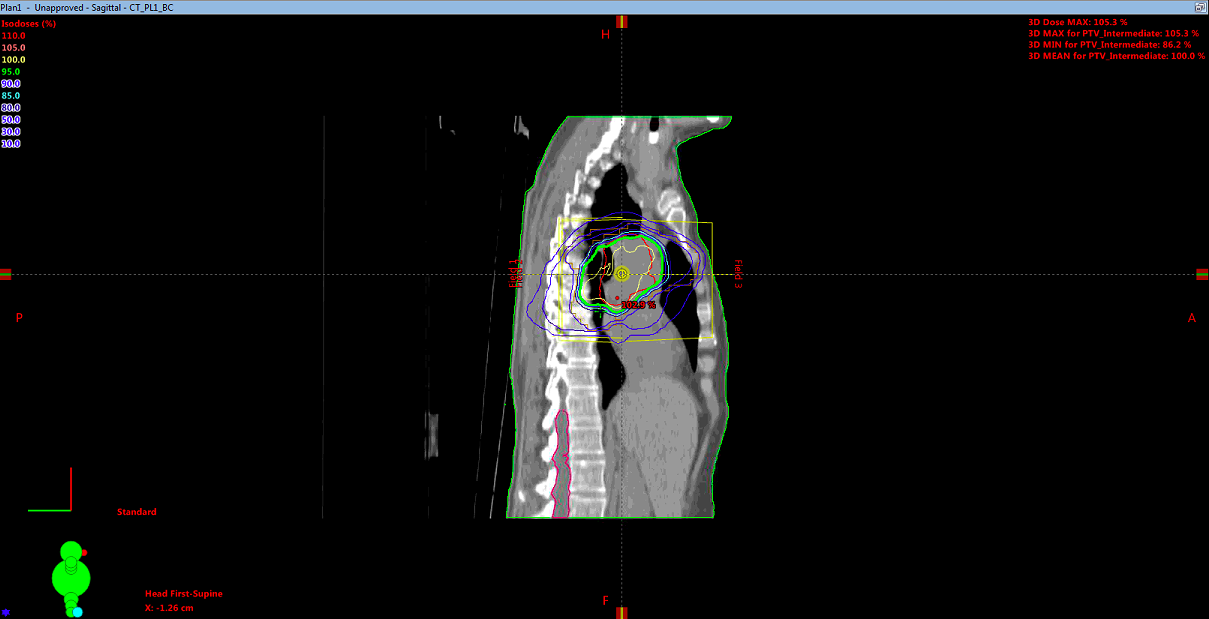
\includegraphics[width=\linewidth]{Bilder/Lunge1_X}
	\caption{Darstellung der Dosisverteilung in der Sagittalansicht der Lunge.}
	\label{fig:lunge1x}
\end{figure}

\begin{figure}[H]
	\centering
	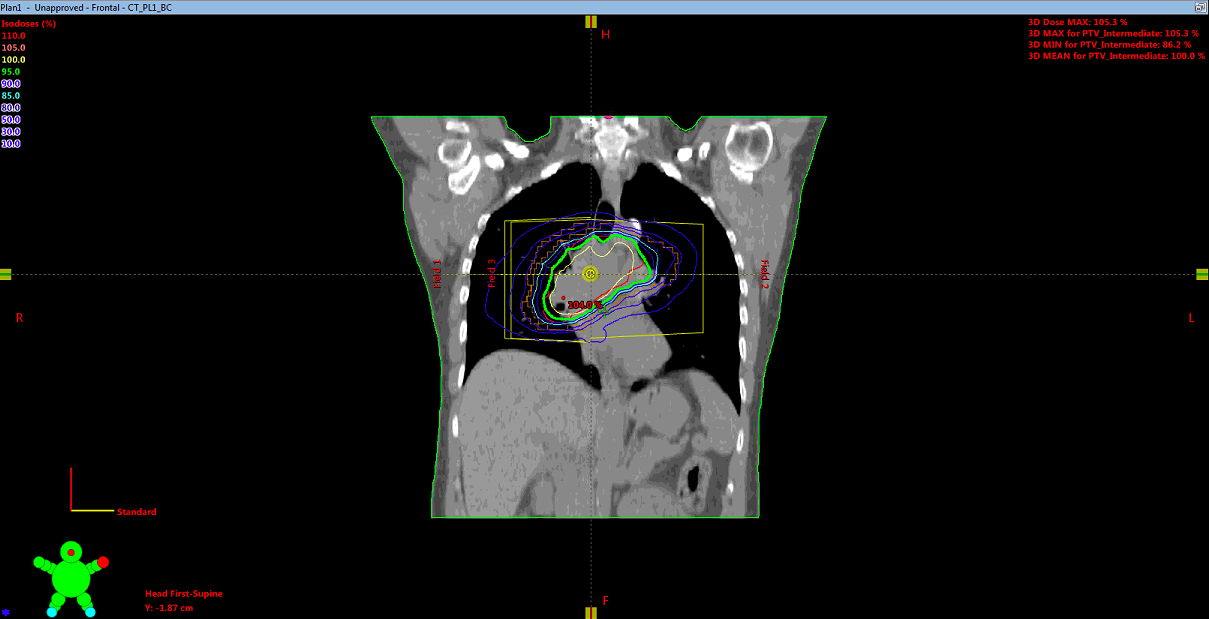
\includegraphics[width=\linewidth]{Bilder/Lunge1_Y}
	\caption{Darstellung der Dosisverteilung in der Frontalansicht  der Lunge.}
	\label{fig:lunge1y}
\end{figure}

\begin{figure}[H]
	\centering
	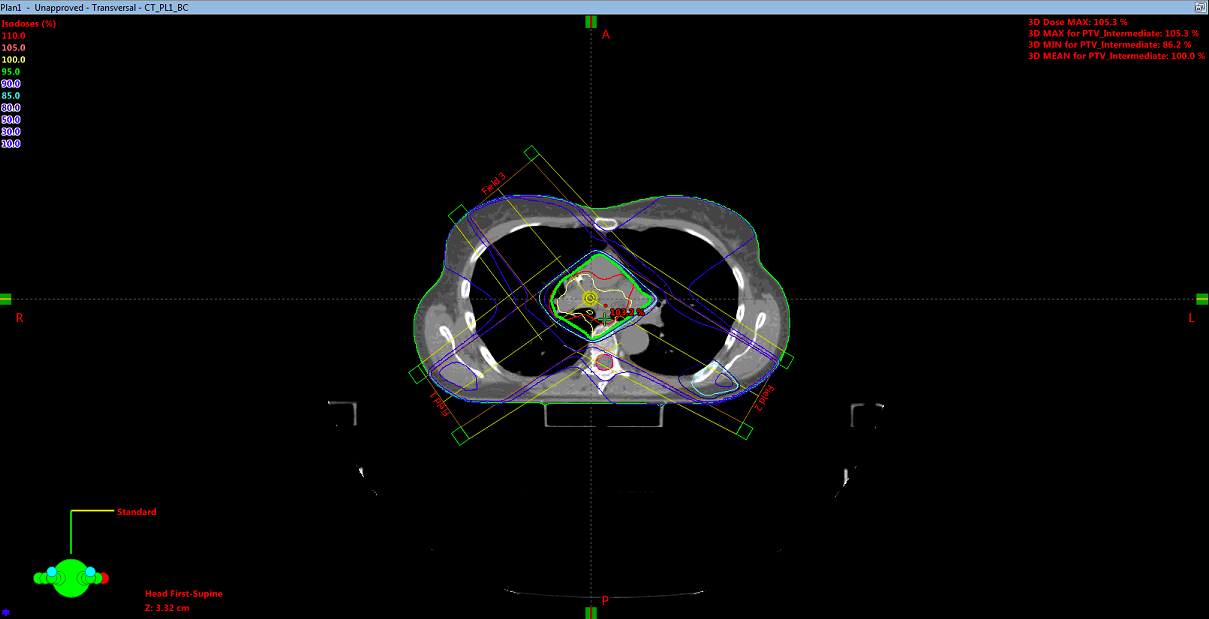
\includegraphics[width=\linewidth]{Bilder/Lunge1_Z}
	\caption{Darstellung der Dosisverteilung in der Transversalansicht  der Lunge.}
	\label{fig:lunge1z}
\end{figure}

\subsection*{Bestrahlungsplan für das PTV2}
Bei dem zweiten Bestrahlungsplan wird das kleinere PTV2 bestrahlt. Bei dieser zweiten Serie ist die applizierte Gesamtdosis auch deutlich geringer als bei der ersten Serie. Die resultierende Dosisverteilung ist in den Abbildungen \ref{fig:lunge2x}, \ref{fig:lunge2y} und \ref{fig:lunge2z} gezeigt. Dabei sind die gleichen Ansichten gezeigt, wie bei dem ersten Plan.
Auch hier wurde nicht geschafft, dass die $\SI{95}{\percent}$-Isodosenlinie nicht $\SI{100}{\percent}$ des PTVs umschließt, sondern nur $\SI{94,1}{\percent}$. Es müssen hier auf die applizierten Dosen berücksichtigt werden, weil sich diese mit der Dosis aus der ersten Serie summieren. Die maximale Dosis des PTVs ist innerhalb des PTVs und liegt bei $\SI{106.3}{\percent}$, also liegt unterhalb der erlaubten maximalen Dosis von $\SI{107}{\percent}$. Die minimale Dosis liegt bei $\SI{87.3}{\percent}$. Diese Dosis liegt minimal unterhalb des gewünschten Dosis von $\SI{95}{\percent}$.
Das zugehörige DVH ist in der Abbildung \ref{fig:lunge2dvh} gezeigt.

\begin{figure}[H]
	\centering
	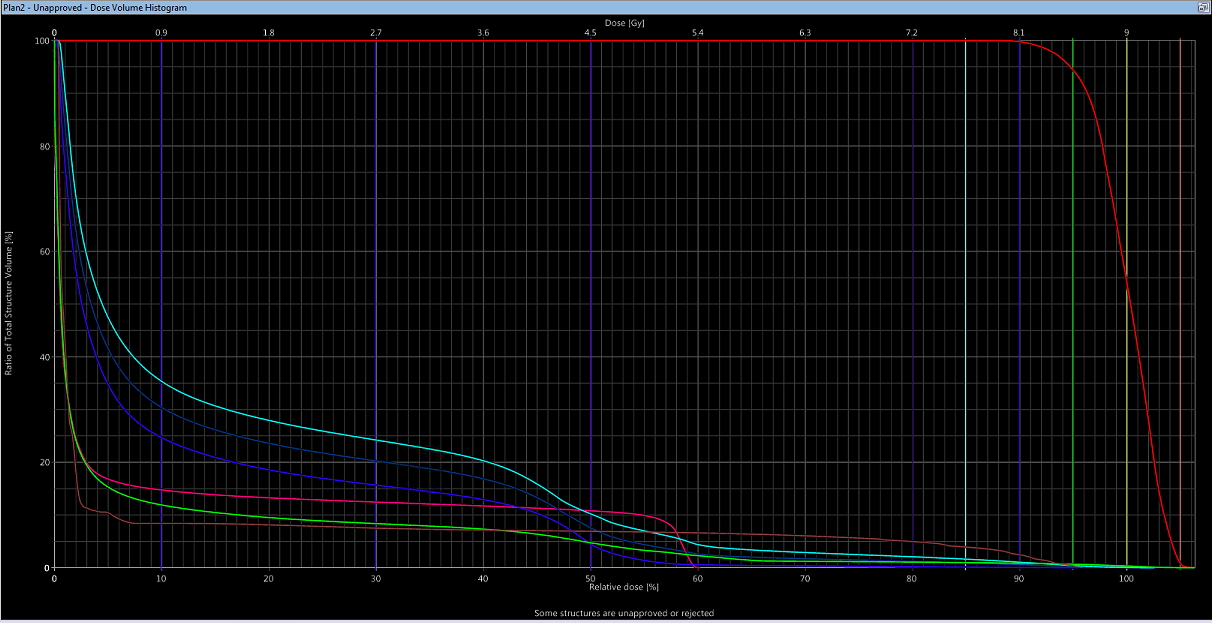
\includegraphics[width=\linewidth]{Bilder/Lunge2_DVH}
	\caption{Zu sehen ist das DVH der Lunge. In roter Farbe dargestellt ist das PTV2 und in grüner Farbe ist der Body. Außerdem sind noch die einzelnen Isodosenlinien eingezeichnet und die einzelnen Kurven zu den Risikoorgane wie z.B. Herz(gelb), Lunge(dunkelblau), die Speiseröhre(braun) und das Rückenmark(pink).}
	\label{fig:lunge2dvh}
\end{figure}

Anhand des DVHs des gesamten Körpers (grüne Kurve) ist zu erkennen, dass der Körper nur eine relativ geringe Dosis deponiert wird. Nur etwa $\SI{4,58}{\percent}$ des Körpervolumens erhält noch eine relative Dosis von $\SI{50}{\percent}$. Im folgenden wird die Summe der beiden Pläne betrachtet um beurteilen zu können ob die Organdosisgrenzwerte eingehalten worden sind.

\begin{figure}[H]
	\centering
	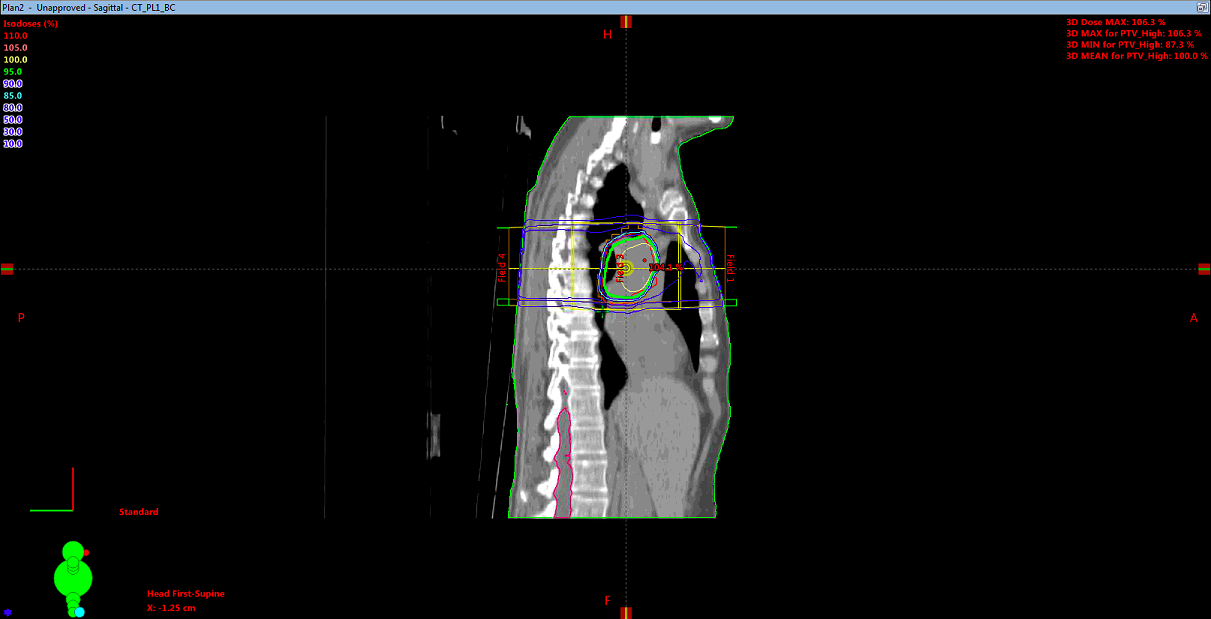
\includegraphics[width=\linewidth]{Bilder/Lunge2_X}
	\caption{Darstellung der Dosisverteilung in der Sagittalansicht der Lunge.}
	\label{fig:lunge2x}
\end{figure}

\begin{figure}[H]
	\centering
	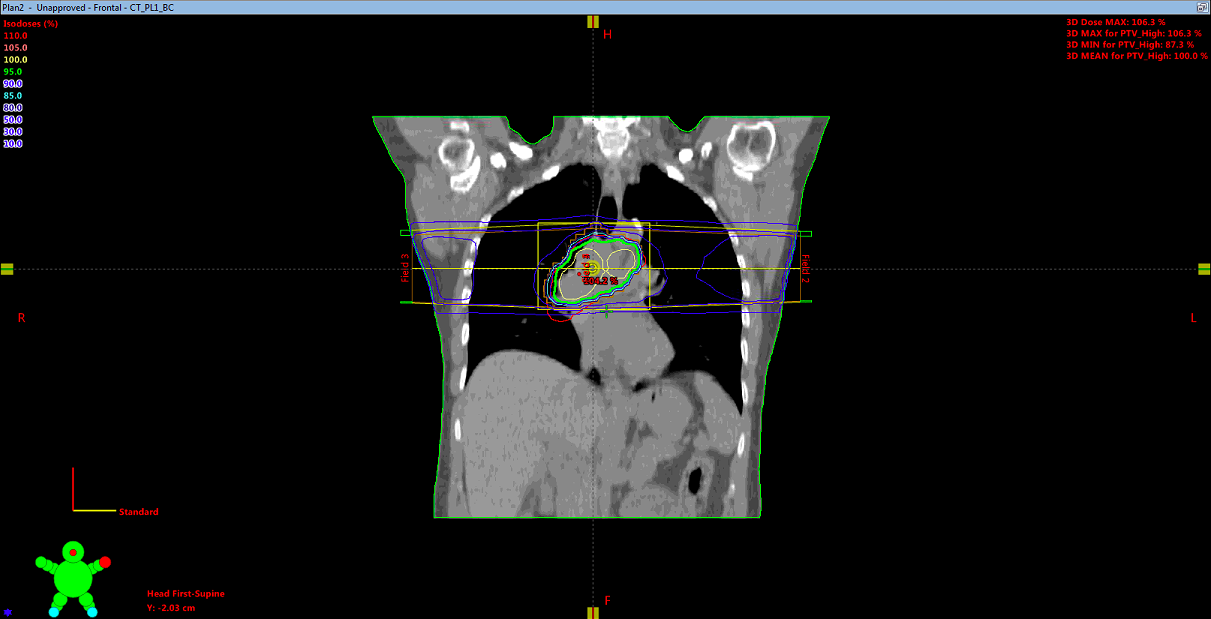
\includegraphics[width=\linewidth]{Bilder/Lunge2_Y}
	\caption{Darstellung der Dosisverteilung in der Frontalansicht der Lunge.}
	\label{fig:lunge2y}
\end{figure}

\begin{figure}[H]
	\centering
	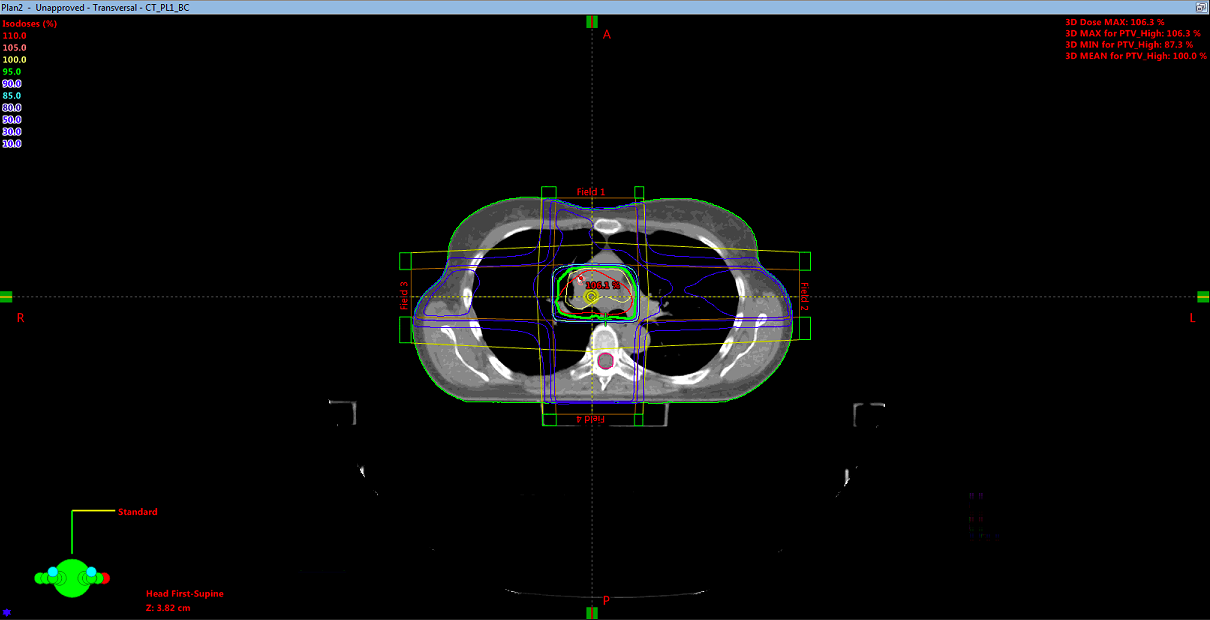
\includegraphics[width=\linewidth]{Bilder/Lunge2_Z}
	\caption{Darstellung der Dosisverteilung in der Transversalansicht der Lunge.}
	\label{fig:lunge2z}
\end{figure}


\subsection*{Summe der Bestrahlungspläne}
In der Abbildung \ref{fig:lunge2dvh} ist das DVH der Summe der beiden Bestrahlungspläne dargestellt. Die Organdosisgrenzwerte werden aus der QUANTEC Tabelle entnommen. Der mittlere Grenzwert für die Lunge beträgt $\SI{20}{\gray}$ und es ist vorgeschrieben, dass $\SI{30}{\percent}$ des Lungenvolumens die maximale Dosis von $\SI{20}{\gray}$ nicht überschreiten darf. Dies wurde erfolgreich eingehalten, weil nur $\SI{25.76}{\percent}$ mit einer Dosis von $\SI{20}{\gray}$ bestrahlt wird.
Der mittlere Grenzwert für das Herz beträgt $\SI{26}{\gray}$ und es ist vorgeschrieben, dass $\SI{46}{\percent}$ des Herzenvolumens die maximale Dosis von $\SI{30}{\gray}$ nicht überschreiten darf. Dies wurde auch erfolgreich eingehalten, weil nur $\SI{3.7}{\percent}$ mit einer Dosis von $\SI{30}{\gray}$ bestrahlt wird.
Die maximale Dosis für das Rückenmark beträgt $\SI{45}{\gray}$ und darf nicht überschritten werden. In dem Fall beträgt die maximale Dosis der Rückenmarks $\SI{31.92}{\gray}$.
Insgesamt wurden bei dieser Bestrahlungsplanung relativ viele Felder erwendet um eine akzeptable Dosisverteilung zu erreichen. Durch die Verwendung von MLCs ist es gelungen die Organdosisgrenzwerte der Lunge, des Herzens und des Rückenmarks nach QUANTEC nicht zu überschreiten.

\begin{figure}[H]
	\centering
	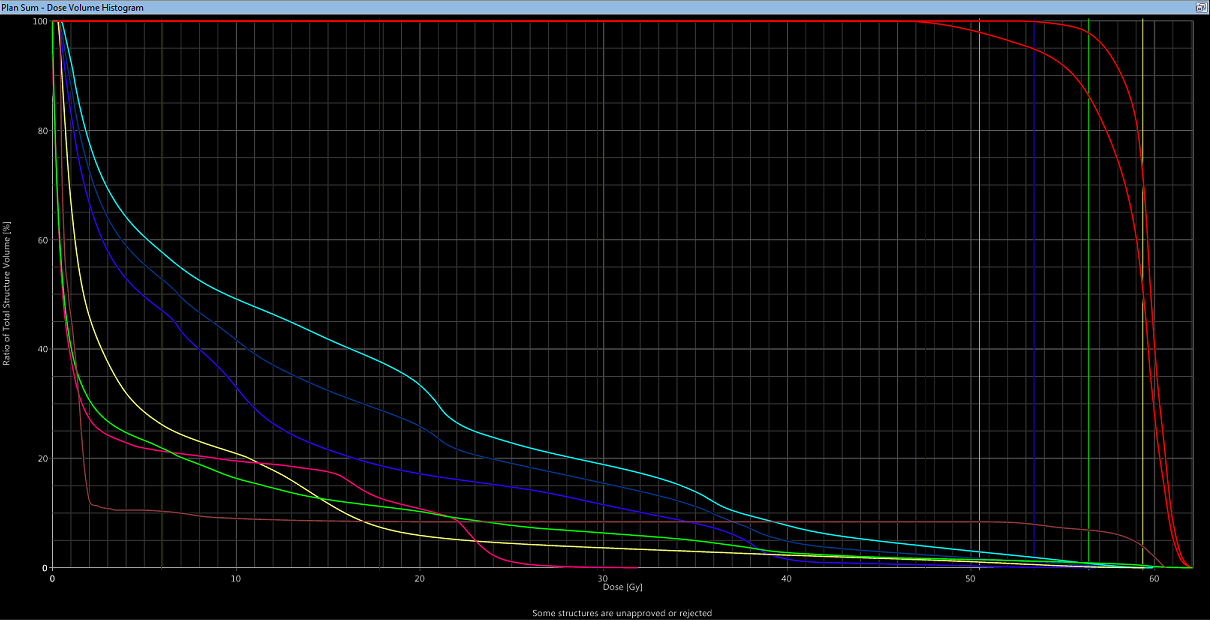
\includegraphics[width=\linewidth]{Bilder/Lunge_DVHsum}
	\caption{DVH für die Summe der beiden Bestrahlungspläne. Für das PTV1 und PTV2 in rot und den gesamten Körper in grün. Außerdem ist das DVH für das Herz in gelb, für die Lunge in dunkelblau, für die Speiseröhre in braun und für das Rückenmark in pink.}
	\label{fig:lungedvhsum}
\end{figure}
